\documentclass[small,algo]{dushClass}


\title{TP -- Spring}
\subtitle{Initialisation aux Frameworks}

\begin{document}

%%%%%%%%%%%%%%%%%%%%%%%%%%%%%%%%%%%%%%%%%%%%
%% SUJET
\section{Sujet}

\subsection{Objectifs}

Dans ce TP, nous reprendrons \emph{la bibliothèque} du précédent TP afin de lui rajouter une couche métier (business). Il se décomposera en 2 parties : 
\begin{itemize}
\item Séparation des préoccupations et injection de dépendances
\item Coupage de \emph{Spring} à \emph{Hibernate} pour réaliser la couche DAO.
\end{itemize}

\subsection{Modèle de données}

Le modèle de données, présenté figure \ref{model} \vpageref{model}, est le même que dans le TP sur Hibernate (section : \emph{pour aller plus loin}). Lui sont ajoutés l'aspect d'exemplaire (\texttt{BookCopy}), et d'emprunt (\testtt{Customer}).

\subsection{Cas étudiés}

Nous allons étudier 2 cas fonctionnels :
\begin{itemize}
\item Création d'une nouvelle référence et ajout d'exemplaires
\item Emprunt d'un exemplaire par un client%si pas déjà 3 locations...
\end{itemize}

\subsubsection{Nouvelle référence}
L'ajout d'une nouvelle référence et d'exemplaires liés suis la procédure ci-après :
\begin{enumerate}
\item\label{add-ihm} L'administrateur renseigne l'identifiant de la libraire et les données sur le livre qu'il souhaite ajouter (code ISBN du livre, titre, description, nombre de pages), ainsi que le nombre d'exemplaires.
\item Recherche de la librairie par son identifiant, elle doit exister
\item Vérification que la référence n'existe pas déjà (par son code ISBN), sinon la référence est mise à jour
\item Génération d'un code pour chacun des exemplaires
\item Sauvegarde de la référence \texttt{Book}, et des exemplaires, en BDD.\\
\end{enumerate}

Le point \ref{add-ihm} ne fait pas partie du TP. Il sera simulé dans la fonction \texttt{main}.

\subsubsection{Emprunt d'un exemplaire}

Pour emprunter un exemplaire, le processus est :
\begin{enumerate}
\item L'utilisateur indique son code client et le code de l'exemplaire qu'il souhaite emprunter
\item le client et l'exemplaire sont recherchés en base, ils doivent exister.
\item vérifications : l'exemplaire n'est pas déjà emprunté, le client ne doit pas avoir plus de 3 emprunts en cours
\item ajouter l'exemplaire à la liste des emprunt en cours du client\\
\end{enumerate}

Le nombre d'exemplaires autorisés doit être configuré dans un fichier \emph{properties}.

\subsection{Architecture}
L'architecture logicielle suit le principe de la \emph{Séparation des Préoccupations}. Elle est présentée figure \ref{tp-spring-soc} \vpageref{tp-spring-soc}.\\

\begin{figure}[ht]\label{tp-spring-soc}
	\center
	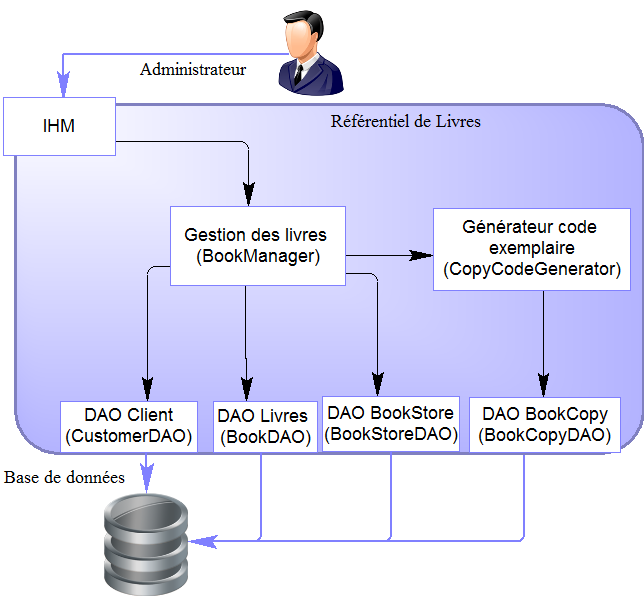
\includegraphics{images/tp-spring-soc.png}
	\caption{Architecture des objets métiers}
\end{figure}

Les briques logicielles sont :
\begin{description}
\item[BookManager] contient les règles métiers telles qu'elles sont décrites dans le cas présentés.
\item[CopyCodeGenerator] Générateur des codes exemplaires
\item[BookDAO] couche d'accès aux données \texttt{Book} de la BDD.
\item[CustomerDAO] couche d'accès aux données \texttt{Customer} de la BDD.
\end{description}


\subsection{Composants fournis}
Afin de gagner du temps, certains composant ont déjà été créés.

\subsubsection{Contexte Spring}
La configuration principale de Spring est dans le fichier : \texttt{src/main/resources/spring/books-context.xml}.\\

Dans la fonction \texttt{main}, le contexte est déjà instancié et est prêt à l'utilisation comme l'était la \texttt{SessinFactory} d'Hibernate lors du premier TP.

\subsubsection{Mapping relationnel}
Le modèle a été poussé jusqu'à sa version "\emph{Pour aller plus loin}" du premier TP. Le mapping est déjà réalisé ainsi que la configuration par Spring.\\

Cette configuration est faite dans le fichier Spring : \texttt{src/main/resources/spring/books-persistence.xml}.

\subsubsection{Interfaces}
Les interfaces de chaque brique ont été crées. Comme dans la convention de nommage utilisée dans le Référentiel Coordonnées, elles commencent par un "\emph{I}" ("i" majuscule).


\subsubsection{Couche DAO bouchonnée}
Une fausse implémentation de la couche DAO est présente dans le package \texttt{net.yvesrocher.training.frameworks.dao.mock}. Celle-ci utilise des \texttt{HashMap} en interne pour simuler une véritable base de données.\\

Pour activer cette couche bouchonnée, il faut ajouter le fichier de configuration \emph{Spring} : \texttt{src/main/resources/spring/books-dao-mock.xml}.



%%%%%%%%%%%%%%%%%%%%%%%%%%%%%%%%%%%%%%%%%%%%
%% DI
\section{Première Partie : Injection de Dépendances}


\subsection{Déclaration des beans et injection}

\subsubsection{Premier bean}

Dans cette partie :
\begin{enumerate}
\item Créez une implémentation à l'interface \texttt{IBookManager}
\item Déclarez la comme un \emph{Bean}\footnote{Rappel : un \emph{bean} est le nom d'une "brique applicative" pour Spring.}
\item Récupérez une instance à partir du contexte Spring\\
\end{enumerate}

Vous pouvez récupérer plusieurs \texttt{IBookManager} et vérifier que ce soit la même instance\footnote{Réalisation d'un classe (exemple : voiture). A ne pas confondre avec une classe qui correspondrait aux plans de la voiture.} qui est renvoyée.\par
Il est possible de modifier le scope en \texttt{singleton}, puis en \texttt{prototype} pour constater des différences de comportement.

\subsubsection{Première dépendance}

Le \emph{BookManager} ne peut pas travailler seul. Il a besoin du générateur de code d'exemplaire, et de la couche d'accès aux données des livres et des clients.\\

Dans un premier temps, nous ne nous intéresseront qu'au générateur : 

\begin{enumerate}
\item Créez une implémentation de l'interface \texttt{ICopyCodeGenerator}
\item Déclarez la comme un \emph{Bean}
\item Injectez un ICopyCodeGenerator dans le \emph{BookManager}
\end{enumerate}


\subsection{Implémenter les beans}

\subsubsection{CopyCodeGenerator}

Implémentez les méthodes du bean \texttt{CopyCodeGeneratorImpl}.\\

Il doit utiliser le \texttt{BookDAO} pour trouver un code disponible.

\subsubsection{BookManager}
Implémentez la méthode \texttt{BookManagerImpl.createNewBook}. Il doit utiliser le \texttt{CopyCodeGenerator} et le \texttt{BookDAO}.

\subsubsection{Tester}

Des méthodes statiques sont présentes sur les DAO afin de lister le contenu de la base de données.





%%%%%%%%%%%%%%%%%%%%%%%%%%%%%%%%%%%%%%%%%%%%
%% DAO
\section{Seconde Partie : Couche d'Accès aux Données}
% Spring + Hibernate

\subsection{Configuration du contexte Spring}

Avant tout, il faut configurer Spring pour qu'il puisse injecter la \texttt{SessionFactory}. Un fichier de configuration est prêt : \texttt{src/main/resources/spring/books-dao-hibernate.xml}. Ajoutez le à la liste lors de la création du contexte Spring.\\

Les nouveaux beans utilisant hibernate risquent de rentrer en conflit avec les bouchons. Retirez le fichier \texttt{src/main/resources/spring/books-dao-mock.xml} de la liste des fichiers de configuration.

\subsection{Ré-implémenter la couche DAO}

Ré-implémenter la couche DAO en utilisant Hibernate.



\subsubsection{Injection de la session factory}

La session factory est maintenant injectable :
\begin{lstlisting}
@Named
public class EmployeeDAOImpl implements IEmployeeDAO {
	
	@Inject
	private SessionFactory factory;
}
\end{lstlisting}


\subsubsection{Ouverture de la session}
La session est ouverte automatiquement lors de l'ouverture d'une transaction. On respecte le pattern : \emph{1 transaction = 1 session}.\\

% pas dans le RC : open session in view.


\end{document}














































